% English draft based on sections/09_social_blockchain_ja.tex
\section{Social Blockchain: Distributed $L_E$ as $\Phi_{\text{net}}$}

\noindent\textbf{Scope of the account.} Social blockchain retains its nontechnical, model-local naming. Network operation and historical sequence are proposed interpretations, not an implemented consensus protocol or a progress law. Git/social cost contrasts are hypotheses without common measured costs. Legitimacy's dependence on social acceptance does not establish principled noncomputability. Individual creation versus social stabilization is a role hypothesis, not an exclusive law of creativity. Independent criteria for records, legitimacy, creation, and shared stopping remain open.

Throughout this chapter, including its summary and historical figure, social logs and distributed stopping are assessed at their declared network scope, not automatically as an individual's LR or LE. Shared records are not all generated history, and a network's retention does not certify any member's role or ownership. Section 5's support, role, and evidence distinctions qualify this architectural comparison without establishing a synchronization mechanism.


\S{}6--\S{}8 described environmental installation, central compression, and long-term maintenance of stopping. This chapter describes a form that maintains stopping without reducing it to a single authority: distributed social stopping. This is called social blockchain.

The term is structural. It does not refer to cryptocurrency or to a specific distributed-ledger implementation. What is borrowed is only the structural feature: distributed nodes form provisional consensus without a single central authority, while keeping the consensus revisable.

\subsection{Structure}

The central feature of social blockchain is the coexistence of stopping and updating without a single authority. Individual nodes generate provisional stops. Logs preserve the history of judgments and their grounds. Forks represent divergent stopping candidates. Merges and abandonments reorganize stopping.

The contrast with technical version control is qualitative. Branching, merging, and rollback are compared with social division, consensus, and revision, without establishing universal cost differences or an inverse cost law.

The center is therefore not Version Control but Consensus.

\subsection{Legitimacy Rather Than Consistency}

Technical blockchains address consistency: can distributed nodes agree on a non-contradictory state? Social blockchain addresses legitimacy: can a distributed stopping point be accepted as legitimate?

Legitimacy is proposed as dependent on time, responsibility, historical acceptance, and distributed recognition. This does not establish principled noncomputability; its relation to revisable stopping remains a structural hypothesis.

\subsection{Creation and Stabilization}

Individual creation and social stabilization form a role hypothesis, not an exclusive division. Relating an individual $L_F$ near a quasi-closure boundary to new concepts, followed by social acceptance or revision, remains a proposed mechanism rather than an established causal sequence.

Individual creation and stabilization through $\Phi_{\text{net}}$ are compared as distinct proposed roles, not as an exhaustive division.

\subsection{Position in the Three-Layer Dynamics}

Social blockchain is a form of $\Phi_{\text{net}}$: the explicit distributed operation of inter-individual $L_E$ networks.

\S{}6--\S{}8 can now be positioned as a sequence. Animism distributes $L_E$ into the environment. God centralizes $L_E$. Religion maintains centralized $L_E$ across generations. Social blockchain operates the $L_E$ network itself without centralizing it.

\begin{figure}[H]
\centering
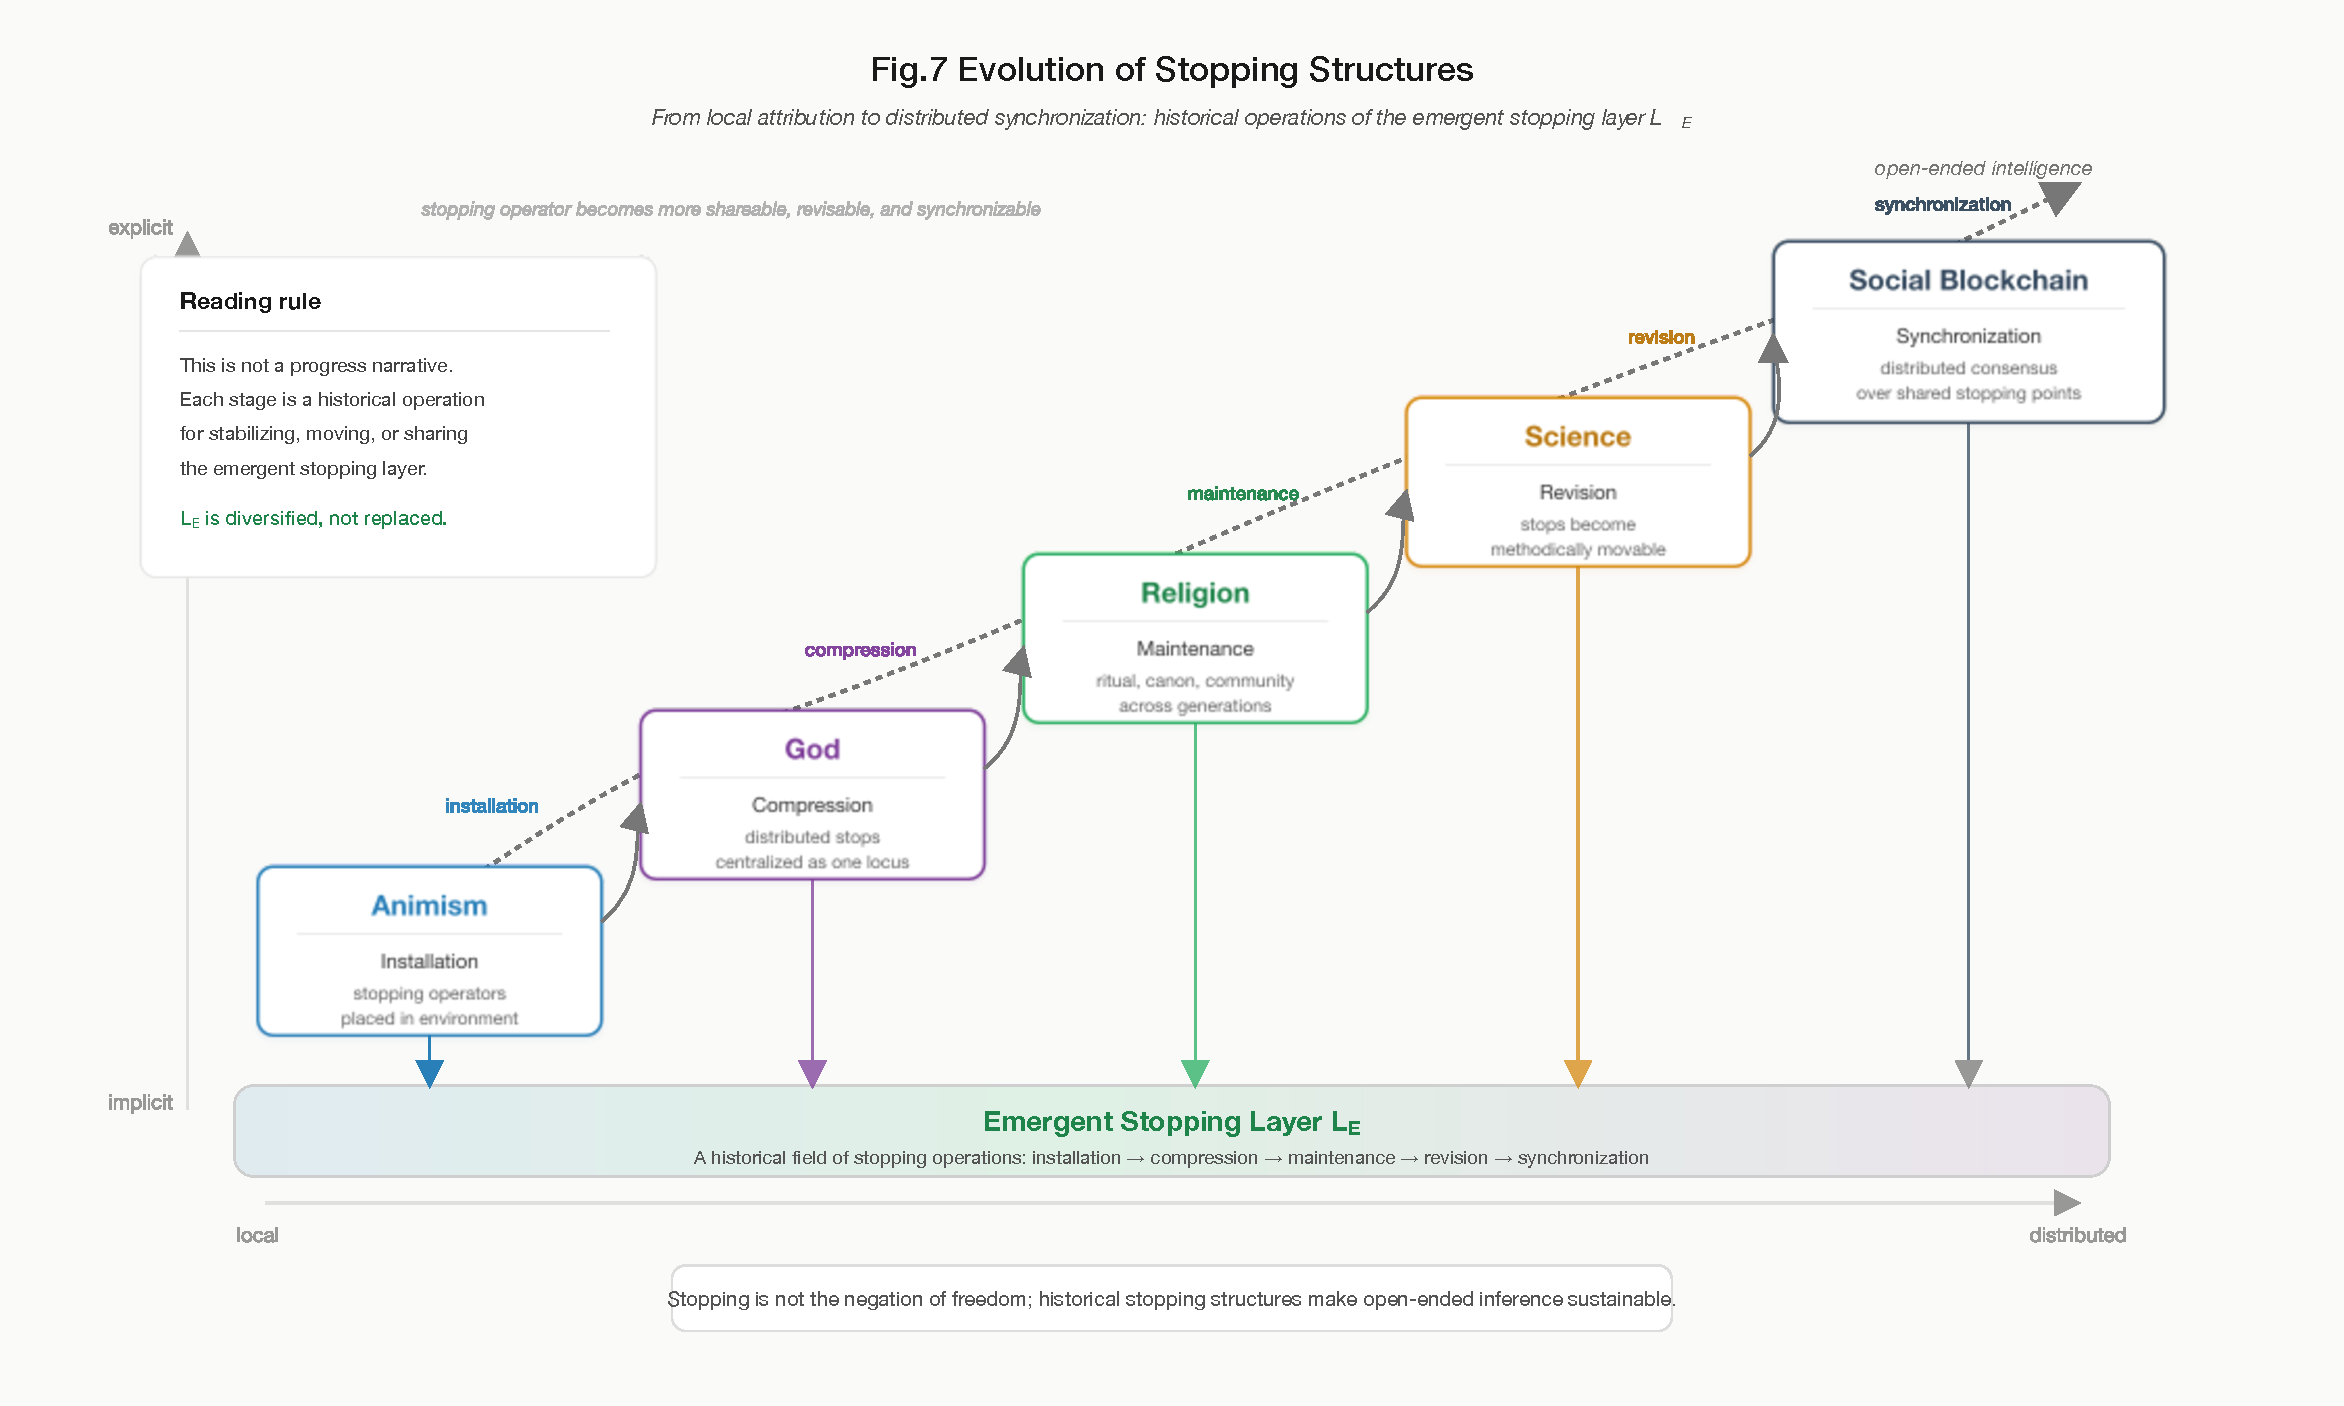
\includegraphics[width=\linewidth]{fig7_evolution_of_stopping_structures.pdf}
\caption{Proposed historical reading of stopping structures. Animism, God, religion, science, and social blockchain are different operations for stabilizing, moving, revising, and synchronizing the model-local stopping role $L_E$, without identifying one common historical object.}
\label{fig:part2-stopping-evolution}
\figurenote{Installation, compression, maintenance, revision, and synchronization are proposed roles of $L_E$, not a verified historical sequence.}{Stopping and open-ended inference are compared functionally. This does not establish a persistence mechanism or a necessary condition for freedom.}
\end{figure}

If religion institutionalizes the long-term maintenance of stopping structures, science can be understood as the operating form that institutionalizes their revision. Social blockchain is compared with these as a proposed role for sharing and synchronization, not placed above them in a validated historical sequence.

\subsection{Bridge to the Gettier Problem}

In social blockchain, stopping is not guaranteed by truth. It is established through distributed acceptance and structural stability. This raises the next question: if social stopping does not guarantee truth, what is knowledge? The Gettier problem is treated in \S{}10 as a structural diagnosis of this gap.

\bigskip
